\tightsection{Design of Dante}

This section presents a detailed system design of Dante.
We begin by formulating the underlying video quality optimization
problem of Dante (\S\ref{subsec:objectives}), and then present a 
simple and efficient control logic that approximately optimizes 
the problem (\S\ref{subsec:logic}), and finally describe a 
prototype implementation of Dante (\S\ref{subsec:impl}) which we
use for evaluation (\S\ref{sec:eval}).

\tightsubsection{Optimization goals}
\label{subsec:objectives}

The high-level goal of Dante is to set the FEC redundancy for
each tile in a given sequence of frames so as to minimize the
average quality degradation of these tiles weighted by the
probability that each tile will be watched by the viewer. 
Dante takes in as input the estimated packet loss rate $p$, 
the sending rate $f$, $m$ frames each having $n$ tiles (we use
$\langle i,j\rangle$ to denote the $j^{\textrm{th}}$ tile of the
$i^{\textrm{th}}$ frame, $0<i\leq m, 0<j\leq n$), the size
$v_{i,j}$ of tile $\langle i,j\rangle$, the probability 
$\gamma_{i,j}$ that tile $\langle i,j\rangle$ will be watched,
and the quality degradation $\delta_{i,j}$ if tile 
$\langle i,j\rangle$ is not recovered, and the maximum delay 
$T$. Then Dante returns as output the FEC redundancy $r_{i,j}$ 
of the $j^{\textrm{th}}$ tile of the $i^{\textrm{th}}$ frame 
($0<i\leq m, 0<j\leq n$). 
Dante's optimization problem can be formulated as following:
\vspace{-0.2cm}
\begin{align}
\textrm{minimize } & \sum_{0<i\leq m}\sum_{0<j\leq n}\gamma_{i,j}d_{i,j}(p,r_{i,j}) \label{eq:obj}\\
\textrm{subject to } & \frac{1}{f}\sum_{0<i\leq m}\sum_{0<j\leq n}v_{i,j}(1+r_{i,j}) \leq T
\label{eq:timeliness}\\
&r_{i,j} \leq 0 \label{eq:positive-redundancy}
\vspace{-0.4cm}
\end{align}
Here, the objective function (Equation~\ref{eq:obj}) is a
weighted sum of the quality degradation over all tiles where 
each tile $\langle i,j\rangle$ is weighted by the probability 
$\gamma_{i,j}$ of it being eventually watched.
Equation~\ref{eq:timeliness} specifies that all the packets
(after encoding redundant packets and the original ones) must 
be sent out before the deadline $T$. 
Dante typically processes all frames in a group of picture 
(GOP) as a batch, in which case 
$T$ is the duration of a GOP. Note that Dante uses 
TCP-Friendly Rate Control algorithm~\cite{TRFC} to compute a
constant sending rate $f$ based on estimated packet loss rate 
and network latency. Finally, 
Equation~\ref{eq:positive-redundancy} ensures the redundancy 
rate is always non-negative.

The key variable here is the quality degradation $d_{i,j}(p,r)$
of tile $\langle i,j\rangle$, if packet loss is $p$ and we use
FEC redundancy $r=\textrm{\# of redundant packets}/\textrm{\# of original packets}$. 
Suppose there are $k$ original packets of a frame, quality
degradation occurs when the lost packets cannot be recovered, 
\ie the number of lost packets $p(r\cdot k+k)$ is greater than
$r\cdot k$, which means $r<\frac{1}{1-p}$. (Note that FEC can
tolerate the loss of {\em any} $r\cdot k$ packet losses.) Therefore, 
\vspace{-0.25cm}
\begin{equation}
d_{i,j}(p,r) = \delta_{i,j}\textrm{, if }r<\frac{1}{1-p}\textrm{; }0\textrm{, otherwise.}\label{eq:degradation}
\vspace{-0.25cm}
\end{equation}

To be more realistic, Equation~\ref{eq:degradation} can be extended
to include one more cause
of quality degradation. Because encoded frames have inherent
dependencies, excessive packet losses can result in quality
degradation on not only one particular frame, but all frames 
whose video decoding depends on it. For instance, losing a ``P'' frame 
will cause all subsequent ``B'' frames, which depend on it, to be lost, even if enough 
of their packets are received. (Note that due to the paramount 
importance of ``I'' frames, we do apply retransmission to 
guarantee the reliability of each ``I'' frame.) To take into 
account the impact of inter-frame dependency on quality 
degradation, we can reformulate quality degradation 
$d_{i,j}(p,r)$ of tile $\langle i,j\rangle$ as a linear 
combination of all previous $d_{i,c}(p,r),0<c\leq i$, \ie
\vspace{-0.25cm}
\begin{equation}
d_{i,j}^{*}(p,r) = \sum_{0<c\leq i}w_{c,i}d_{c,j}(p,r) \label{eq:degradation-new}
\vspace{-0.25cm}
\end{equation}
where $w_{c,i}$ encodes the dependency of frame $i$ on frame $c$. 
More details can be found in~\cite{distortion_model}. 
In the rest of the paper, we use the formulation based on 
Equation~\ref{eq:degradation-new}.




\tightsubsection{Adaptive logic of FEC redundancy}
\label{subsec:logic}


Next, we present Dante's logic that efficiently solves the above 
problem formulation and sets the FEC redundancy of each tile to 
maximize the overall video quality. 

First of all, our problem formulation cannot be
easily tractable. This is because of the non-linearity of 
$d_{i,j}(p,r)$; according to Equation~\ref{eq:degradation}, 
$d_{i,j}(p,r)$ changes sharply depending on whether $r$ is 
greater than $\frac{1}{1-p}$. In fact, we can reduce the problem 
formulation to the ``knapsack problem'' know to be NP-
complete~\cite{NP-complete}. We briefly sketch the 
reduction here. Imagine we have one item for each tile, so in 
total $m\cdot n$ items to be put in a knapsack; if 
$r_{i,j}<\frac{1}{1-p}$ holds for tile $\langle i,j\rangle$, then 
we set the corresponding item to be 0 (\ie not put in the 
knapsack), otherwise, 1 (\ie put in the knapsack). Then our 
minimizer (Equation~\ref{eq:obj}) can be equivalently transformed 
to a maximizer of a linear combination of the binary variables of 
all items, and Equation~\ref{eq:timeliness} can be equivalently 
transformed to a constraint that another linear combination of 
the binary variables must be lower than a threshold. Finally, the 
resulting description---maximizing a weighted sum of some binary 
variables subject to a constraint that another linear combination 
of the binary variables is less than a threshold---is exactly the 
formulation of 0-1 knapsack problem.


\begin{algorithm}[t] 
	\centering 
	\caption{FEC redundancy adaptive algorithm}
	\begin{algorithmic}[1]
	\STATE $B\leftarrow Tf-\sum_{0<i\leq m}\sum_{0<j\leq n}v_{i,j}$  \footnotesize{//Budget of redundant packets}
	\STATE $r_{i,j}\leftarrow 0, 0<i\leq m, 0<j\leq n$  \footnotesize{//Initializing FEC redundancy}
	\WHILE{$B>0$}
		\STATE $\Delta_{max}\leftarrow 0, Tile_{chosen}\leftarrow None$
		\FOR{$i=1,\dots,m$}
			\FOR{$i=j,\dots,n$}
				\STATE $r_{i,j}^{'}\leftarrow r_{i,j}+\frac{1}{v_{i,j}}$ \footnotesize{//Add one redundant packet to tile $\langle i,j\rangle$}
				\STATE $\Delta\leftarrow\gamma_{i,j}d_{i,j}^{*}(p,r_{i,j})-\gamma_{i,j}d_{i,j}^{*}(p,r_{i,j}^{'})$ \footnotesize{//Incremental quality improvement}
				\IF{$\Delta>\Delta_{max}$}
					\STATE $\Delta_{max}\leftarrow\Delta, Tile_{chosen}\leftarrow\langle i, j\rangle$
				\ENDIF
			\ENDFOR
		\ENDFOR
		\STATE $\langle i, j\rangle\leftarrow Tile_{chosen}, r_{i,j}\leftarrow r_{i,j}+\frac{1}{v_{i,j}}$ \footnotesize{//Greedily add the packet to the most needed tile}
		\STATE $B\leftarrow B-1$ \footnotesize{//Reduce budget by one}
	\ENDWHILE
	\RETURN {$r_{i,j}, 0<i\leq m, 0<j\leq n$}
	\end{algorithmic}  
	\label{alg:dante}
\end{algorithm} 

Given that the problem cannot be solve efficiently, we then give 
an heuristic algorithm (shown in Algorithm~\ref{alg:dante}) that 
can solve the problem in linear time and our experimental results 
indicate it results in good performance. The algorithm starts 
with calculating a budget of total number of redundant packets 
$B=Tf-\sum_{0<i\leq m}\sum_{0<j\leq n}v_{i,j}$. Then it greedily assigns 
each redundant packet in the budget to the tile that currently 
maximizes the reduction of quality degradation, \ie 
$\Delta=\gamma_{i,j}d_{i,j}^{*}(p,r_{i,j})-\gamma_{i,j}d_{i,j}^{*}(p,r_{i,j}^{'})$. 
If tile $\langle i, j\rangle$ is chosen, we increment its FEC 
redundancy value by $\frac{1}{v_{i,j}}$ where $v_{i,j}$ is the 
size of the tile. This process continues until we use up all 
redundant packets in the budget.


\begin{figure}[t]
	\centering
	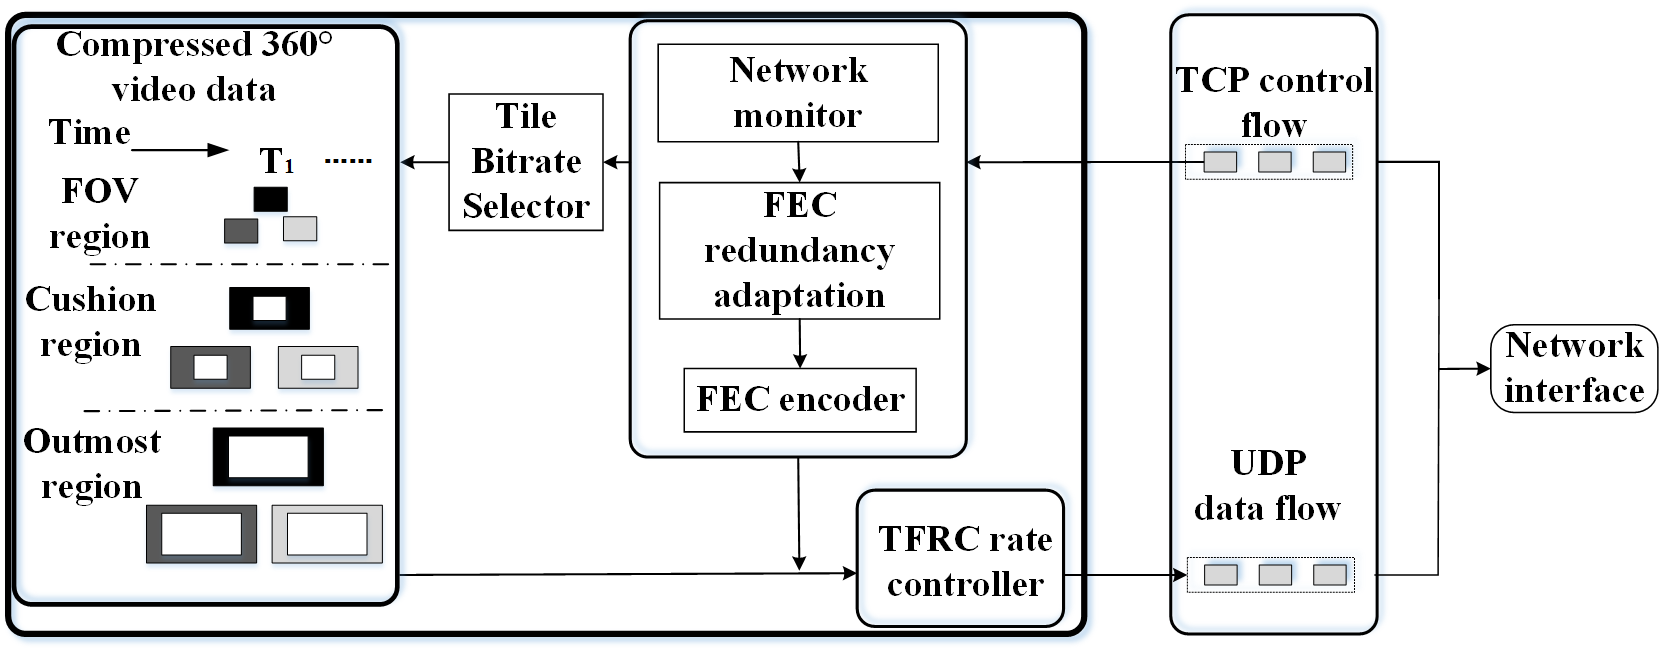
\includegraphics[width=0.5\textwidth]{paper_figs/architecture_dante_0626_v4.png}
	\vspace{-0.3cm}
	\tightcaption{The Architecture of Protocol}
	\label{fig:overview}
\end{figure}




\tightsubsection{Prototype implementation}
\label{subsec:impl}

%\jc{change from client-driven to server-driven!}

We have implemented a prototype of Dante, and here we discuss 
some of its important details. 
Figure~\ref{fig:overview} depicts an overview of the 
implementation. There are two connections between the client and 
the server: one UDP connection to send video data packets, and 
one TCP connection to provide reliable communication of control 
messages, including start/end of a playback session and network information feed (\eg packet loss rate, latency) from receivers. According to the constant network information feed from receivers, the server, at the boundary of each GOP (typically every several seconds), runs Algorithm~\ref{alg:dante} to determine the FEC 
redundancy for the frames and tiles in the next GOP, which then is sent to
 the client. On determining FEC redundancy for frames of the GOP, the server uses 
RS codes to 
inject redundant packets, re-encodes them with the original 
video data packets, and sends the data using TFRC-based sending 
rate. Note that the Dante implementation is complementary to 
application-level bitrate adaptation strategies, and can be 
deployed by replacing the existing underlying transport protocol 
with minimal changes to the video player. 

% Dante is proposed to support high-quality 360-degree video
% streaming service over the wireless network. In Dante, UDP combined with the systematic FEC, RS code, is integrated to provide data delivery service over wireless networks. And only the data of I frames is retransmitted if no ACK is received by the server in time ${T^I}$, in order to guarantee the video data received is decodable by video codec.
% Besides, TCP is supplementary to exchange control information, which is of significance. The overall protocol architecture is illustrated in Figure 2.
